% !TEX root = ../main.tex
\subsubsection{Hadronic Variables}
\label{14.22::hadronic_variables}
    The acceptance of the hadronic variables $z_h$, $p_T^2$, and $\phi_{PQ}$ for $e^-\pi^+$ and $e^-\pi^-$ are presented in Figure \ref{fig::14.22::hadronic_acc}.
    Each one is presented in integrated kinematical region for all electron variables and other hadronic variables.

    % Lower acceptance.
    As can be seen in the figures, acceptance for the hadronic variables is lower than that for electron variables.
    This is to be expected, since they require both the trigger electron and at least one hadron to be accepted by the detector.
    This same effect is seen in the $e^-\pi^+$ and $e^-\pi^-$ entries presented in the efficiency Table \ref{tab::14.14::fmt_efficiency_study}.

    % Particle charge-dependent acceptance.
    Furthermore, the hadronic variables acceptance for $e^-\pi^-$ is shown to be about half of that for $e^-\pi^+$.
    This again is related to the $\theta$ acceptance of CLAS12 which, due to the non-trivial magnetic field of the solenoid, bends the tracks of particles.

    During run 12016, the solenoid field was configured to have a polarity of $-0.75$.
    This in turn causes negative particle tracks to bend inward, towards the low-$\theta$ region of the DC, as explained in Section \ref{14.21::electron_variables}.
    Positive particle tracks, in contrast, bend outward, casting them towards the high-$\theta$ region of the detector.
    The $\phi$ and $\theta$ acceptances of the detector for negative particles can be seen in Figure \ref{fig::14.21::theta_study_neg}, while those for positive particles in shown in Figure \ref{fig::14.22::theta_study_pos}.

    As the plots show, the DC are generally much more receptive to positive particles.
    This means that more $\pi^+$ are going to be detected than $\pi^-$, thus explaining differences in the acceptance of hadronic variables between $e^-\pi^+$ and $e^-\pi^-$.

    % zh.
    $z_h$ has no dependance on the $\theta$ angle of either the hadron or the scattered electron.
    This means that the $z_h$ acceptance ratios that we see in both Figures \ref{fig::14.22::zh_acc_211} and \ref{fig::14.22::zh_acc_-211} are related only to the intrinsic $z_h$ acceptance of CLAS12.

    % pt2.
    $p_T^2$, first described in Section \ref{13.40::acceptance_correction}, is defined as
    \begin{equation*}
        p_T^2 = p_h^2 \cdot \left(1 - \cos^2(\theta_{PQ})\right),
    \end{equation*}
    where $p_h$ is the momentum of the hadron in the lab frame, and $\theta_{PQ}$ is the angle between the virtual interation photon and the detected hadron.
    Both $p_h$ and $\theta_{PQ}$ have a non-trivial dependence on the $\theta$ of both the scattered electron and the detected hadron.
    We can see the variable plotted in Figures \ref{fig::14.22::pt2_acc_211} and \ref{fig::14.22::pt2_acc_-211}.
    % NOTE. A 3D plot with \theta on the x axis, \phi on the y axis, and \theta_PQ on the z axis would be able to disentangle this non-trivial dependence, but that's beyond the scope of this thesis.

    In addition to its shape, we can perceive an increase in both value and uncertainty at $p_T^2 \gsim 1.4$ for both DC and FMT acceptance.
    This is merely a statistical uncertainty, as very few particles with these values of $p_T^2$ are accepted by CLAS12 in the produced simulations.
    This uncertainties will later be inherited by the plots obtained in Section \ref{14.30::study_results}.

    % phipq.
    % NOTE. At the end of the day, the equation would confuse people more than just saying what the variable is, so fuck it we ball.
    $\phi_{PQ}$, as defined in Section \ref{13.40::acceptance_correction}, is the angle between the leptonic and the hadronic planes.
    This variable in particular has a very non-trivial relationship with the $\theta$ and $\phi$ angles of both scattered electron and detected hadron.
    Despite this, we do know that $\phi_{PQ}$ acceptance commonly follows a shape similar to what we see in Figures \ref{fig::14.22::phipq_acc_211} and \ref{fig::14.22::phipq_acc_-211}, as can be seen in DIS analysis publications such as \cite{moran2022}.

    \begin{figure}
        \centering
        % zh pi+.
        \begin{subfigure}[b]{0.49\textwidth}
            \centering
            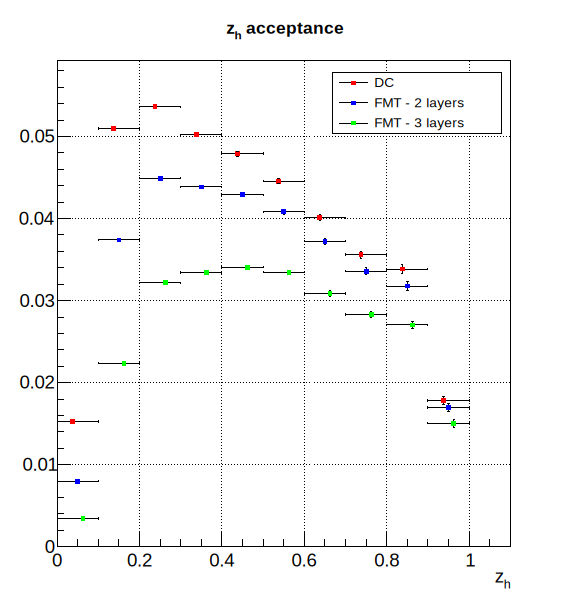
\includegraphics[width=\textwidth]{22zh_acc_211.pdf}
            \caption{$z_h$ acceptance for $e^-\pi^+$.}
            \label{fig::14.22::zh_acc_211}
        \end{subfigure}
        \hfill
        % zh pi-.
        \begin{subfigure}[b]{0.49\textwidth}
            \centering
            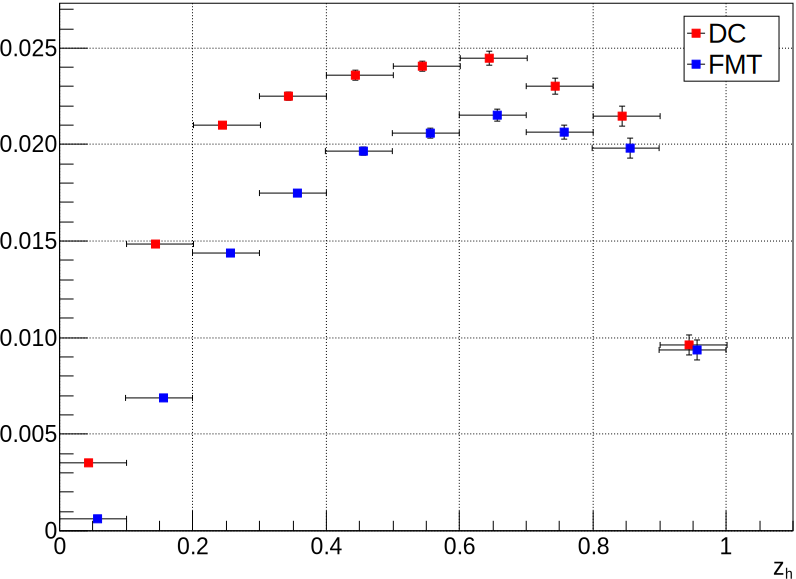
\includegraphics[width=\textwidth]{22zh_acc_-211.pdf}
            \caption{$z_h$ acceptance for $e^-\pi^-$.}
            \label{fig::14.22::zh_acc_-211}
        \end{subfigure}

        \centering
        % pt2 pi+.
        \begin{subfigure}[b]{0.49\textwidth}
            \centering
            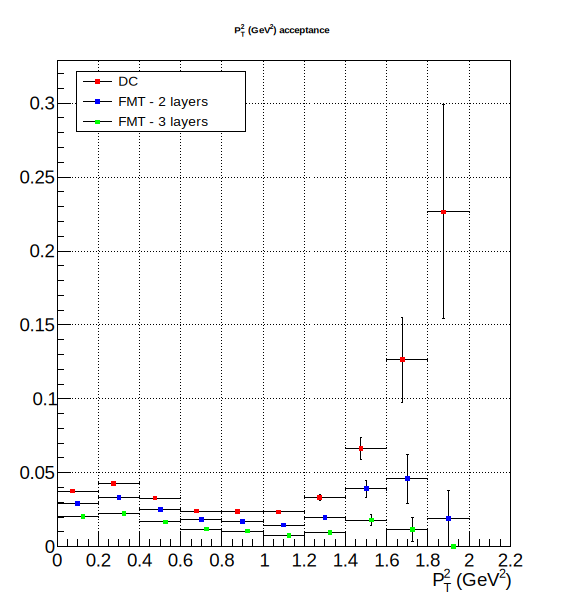
\includegraphics[width=\textwidth]{22pt2_acc_211.pdf}
            \caption{$p_T^2$ acceptance for $e^-\pi^+$.}
            \label{fig::14.22::pt2_acc_211}
        \end{subfigure}
        \hfill
        % pt2 pi-.
        \begin{subfigure}[b]{0.49\textwidth}
            \centering
            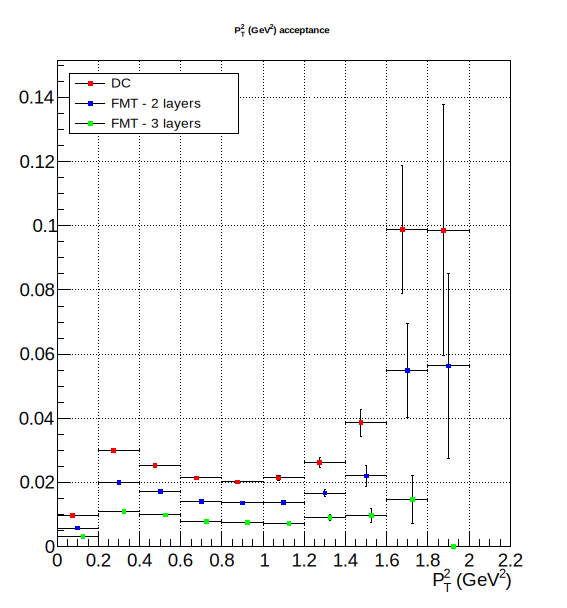
\includegraphics[width=\textwidth]{22pt2_acc_-211.pdf}
            \caption{$p_T^2$ acceptance for $e^-\pi^-$.}
            \label{fig::14.22::pt2_acc_-211}
        \end{subfigure}

        \centering
        % phipq pi+.
        \begin{subfigure}[b]{0.49\textwidth}
            \centering
            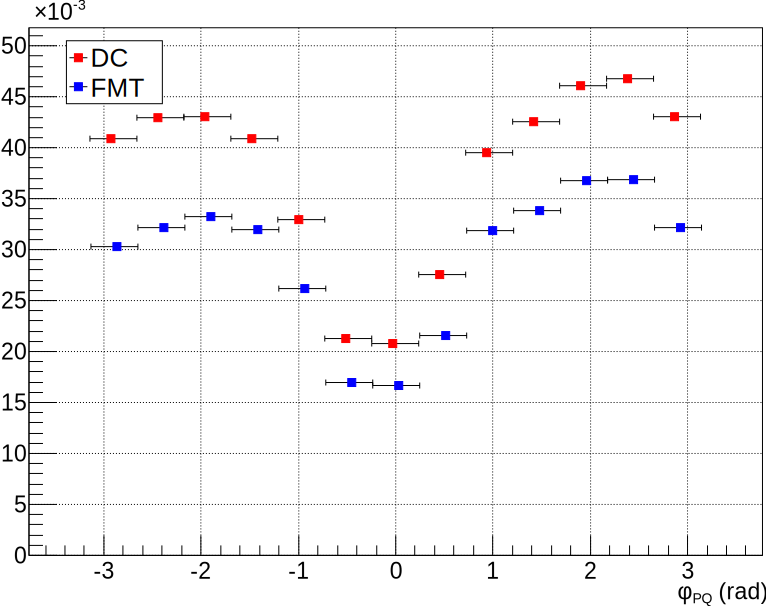
\includegraphics[width=\textwidth]{22phipq_acc_211.pdf}
            \caption{$\phi_{PQ}$ acceptance for $e^-\pi^+$.}
            \label{fig::14.22::phipq_acc_211}
        \end{subfigure}
        \hfill
        % phipq pi-.
        \begin{subfigure}[b]{0.49\textwidth}
            \centering
            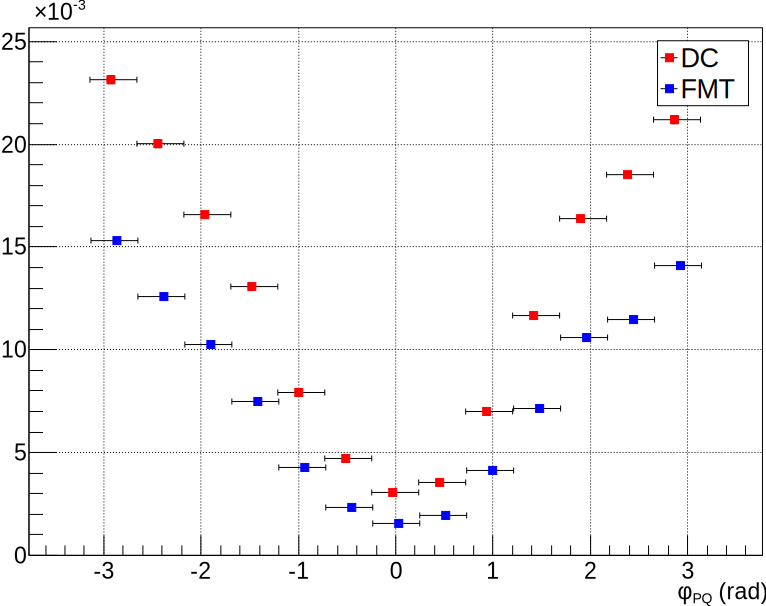
\includegraphics[width=\textwidth]{22phipq_acc_-211.pdf}
            \caption{$\phi_{PQ}$ acceptance for $e^-\pi^-$.}
            \label{fig::14.22::phipq_acc_-211}
        \end{subfigure}
        \caption[hadronic variables acceptance]
        {$z_h$, $p_T^2$, and $\phi_{PQ}$ acceptances for $e^-\pi^+$ and $e^-\pi^-$.
        All electron and other hadronic variables are integrated in all Figures.
        The bin markers are slightly shifted in $x$ to improve legibility.}
        \floatfoot{Source: Own elaboration, using the \href{https://github.com/bleaktwig/clas12-rge-analysis}{clas12-rge-analysis} software.}
        \label{fig::14.22::hadronic_acc}
    \end{figure}

    \begin{figure}
        \centering
        % phi vs theta.
        \begin{subfigure}[b]{\textwidth}
            \centering
            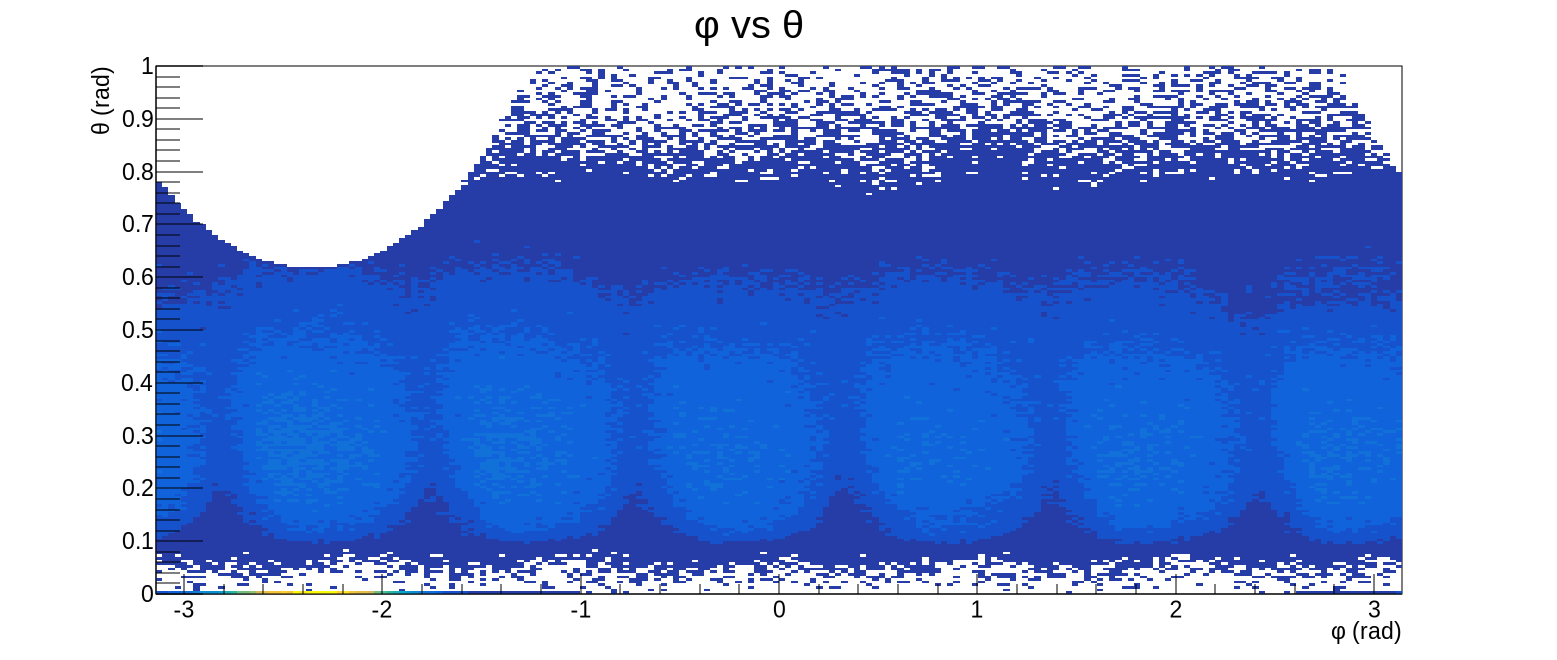
\includegraphics[width=\textwidth]{22phi_theta_pos.pdf}
            \caption[$\phi$ vs $\theta$ for positive particles]
            {$\phi$ vs $\theta$ for positive particles detected by DC.
            The sector with less acceptance than the rest is caused by \textbf{TODO}.}
            \label{fig::14.22::phi_theta_pos}
        \end{subfigure}
        % theta.
        \begin{subfigure}[b]{\textwidth}
            \centering
            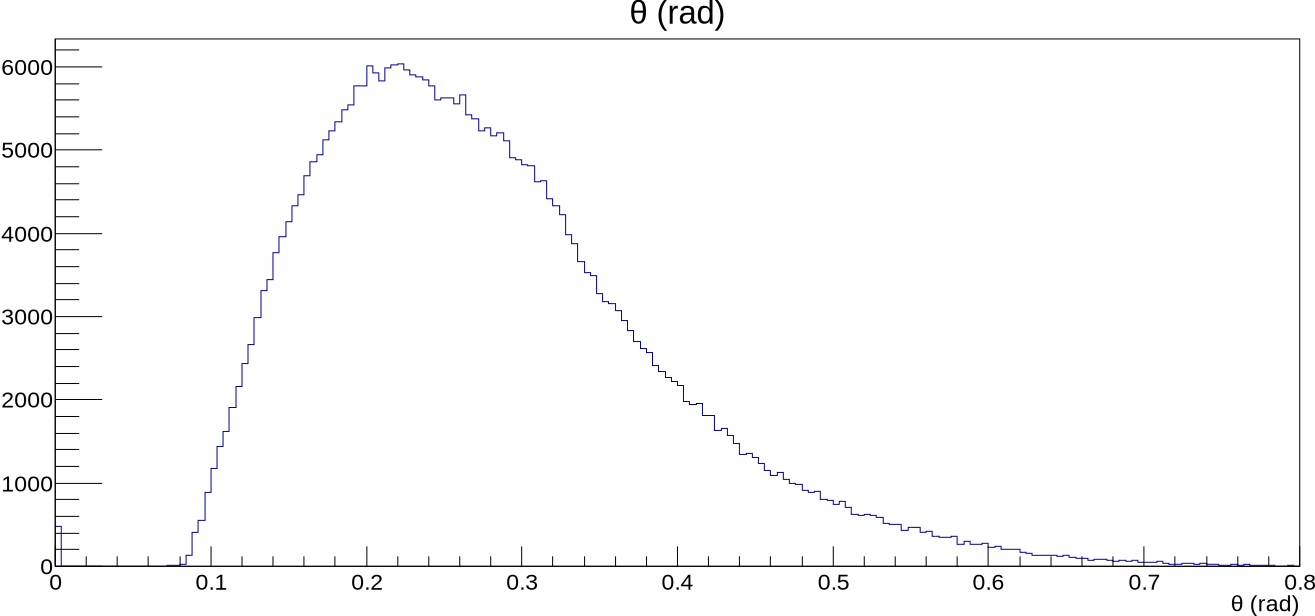
\includegraphics[width=\textwidth]{22theta_pos.pdf}
            \caption[$\theta$ for positive particles]
            {$\theta$ for positive particles detected by DC.}
            \label{fig::14.22::theta_pos}
        \end{subfigure}
        \caption[$\theta$ study for positive particles]
        {$\theta$ study for positive particles.
        Simulated data.}
        \floatfoot{Source: Own elaboration, using the \href{https://github.com/bleaktwig/clas12-rge-analysis}{clas12-rge-analysis} software.}
        \label{fig::14.22::theta_study_pos}
    \end{figure}

    \pagebreak
